\chapter{Técnicas de Diseño}\label{sec-patrones}

\section{Patrones de Diseño}
``Un patrón describe un problema recurrente sobre un ambiente, y entonces describe la técnica que soluciona el problema de forma tal que puede ser utilizado sobre cualquier instancia del problema''\cite{DesignPatterns}, es decir, que dados los requerimientos funcionales del sistema es posible analizar la comunicación entre sus distintas partes y de esta forma saber lo patrones que son útiles para dar solución. Los patrones son organizados en tres categorías\cite{DesignPatterns}:
\begin{itemize}
	\item \textbf{Creacionales}: describen la forma en que las entidades (objetos si se utiliza el paradigma orientado a objetos) del sistema son creadas.
	\item \textbf{Estructurales}: describen la organización entre las entidades del sistema.
	\item \textbf{Comportamiento}: describen la comunicación entre entidades del sistema
\end{itemize}

\section{Patrón Objeto de Acceso a Datos}\label{sec-dao}
El patrón Objeto de Acceso a Datos (DAO por sus siglas en inglés) encapsula y abstrae la conexión a una fuente de datos (archivos de texto plano, bases de datos relacionales, bases de datos no relacionales, etc.) y expone operaciones pertinentes al manejo de tales datos\cite{OCPJavaSE7,OCAPJavaSE7}:
\begin{enumerate}
	\item [] \textbf{buscar}: Realiza la búsqueda de un único elemento, en caso de no encontrarse tal elemento la respuesta es nula.
	\item [] \textbf{listar}: Extrae todos los elementos, el resultado puede utilizar estrategias de paginación.
	\item [] \textbf{insertar}: Guarda un nuevo elemento en la fuente de datos.
	\item [] \textbf{actualizar}: Actualiza la información de un elemento existente en la fuente de datos.
	\item [] \textbf{borrar}: Borra el registro de un elemento en la fuente de datos.
\end{enumerate}


\section{Patrón Modelo-Vista-Controlador}\label{sec-mvc}
Para Sarcar\cite{JavaDesignPatternsExamples} el patrón Modelo Vista Controlador (MVC) es un patrón de arquitectura que consiste de tres grandes componentes: Modelo, Vista y Controlador. El Controlador conduce la comunicación entre la Vista y el Modelo, en la Figura \ref{fig:dia-mvc-simple} se muestra el flujo de comunicación entre los componentes MVC.
\begin{enumerate}
	\item \textbf{Modelo}: tiene la responsabilidad de manejar el acceso a los datos persistentes y la lógica de negocio, usualmente se acompaña del patrón DAO\footnote{Ver sección \ref{sec-dao}} para el manejo de datos.
	\item \textbf{Vista}: es la capa de presentación, es responsable de mostrar los datos al actor\footnote{Puede ser una persona u otro sistema} que use el sistema.
	\item \textbf{Controlador}: es el intermediario entre la Vista y el Modelo: comunica las peticiones de la vista al modelo y los datos del modelo a la vista.
\end{enumerate}
\begin{figure}[h]
  \centering
  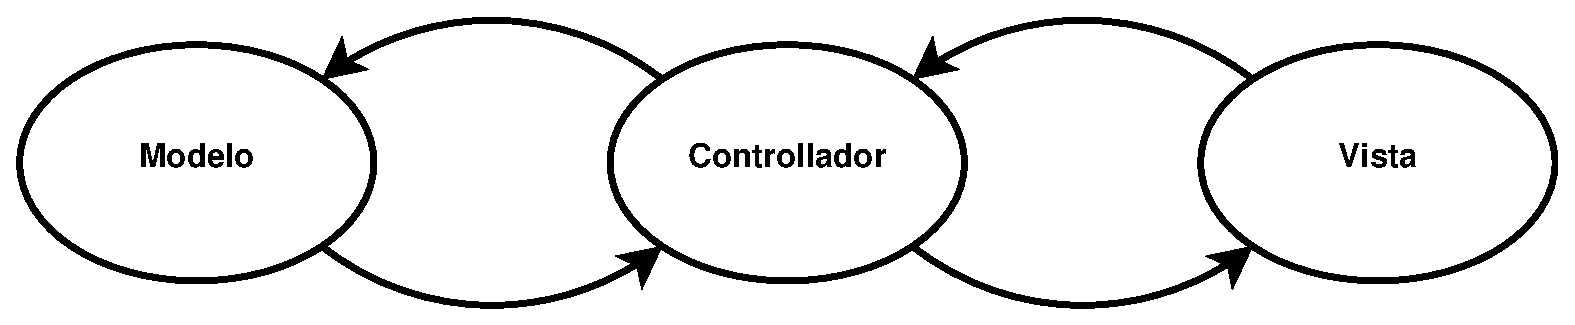
\includegraphics[scale=0.4]{dia-mvc-simple}
  \caption{Diagrama del patrón MVC\cite{JavaDesignPatternsExamples}.}
  \label{fig:dia-mvc-simple}
\end{figure}


\iffalse
\section{Arquitectura 4+1} Organiza cada decisión en el diseño del sistema en cuatro partes llamadas vistas (ver Figura \ref{fig:dia-arq-4-1}), cada vista se encarga de enfocarse en un aspecto del diseño, estas cuatro vistas son unificadas por una cuarta vista de escenarios o casos de uso\cite{ViewModel4plus1}:
\begin{itemize}
	\item \textbf{Vista Lógica}: son las reglas del negocio por las que se rige la operación del usuario final.
	\item \textbf{Vista de Proceso}: refleja concurrencia y sincronización.
	\item \textbf{Vista de Física}: describe las relaciones del software con el hardware.
	\item \textbf{Vista de Desarrollo}: describe la organización estática del software en su ambiente de desarrollo.
\end{itemize}

\begin{figure}[h]
\centering
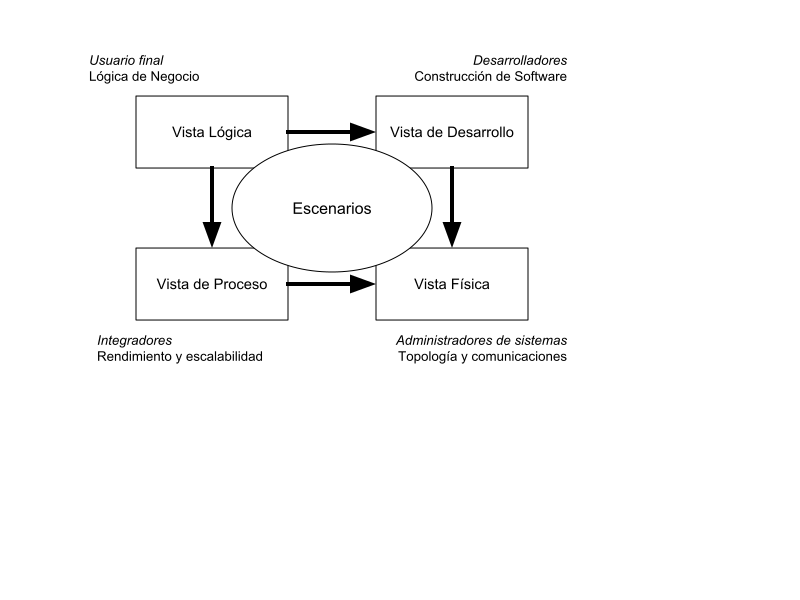
\includegraphics[scale=0.5]{dia-arq-4-1} 
\caption{Diagrama de arquitectura 4+1.\cite{ViewModel4plus1}}
\label{fig:dia-arq-4-1}
\end{figure}


\section{Arquitectura Orientada a Servicios}
Thomas Erl describe la Arquitectura Orientada a Servicios (\textbf{SOA} por sus siglas en inglés) como el modelo arquitectónico del cómputo orientado a servicios\cite{SOAWithRest}, a continuación se muestran las definiciones de Erl sobre los conceptos de Orientación a Servicios:
\begin{quote}
La \textbf{Orientación a Servicios} es el paradigma de diseño dedicado para la creación de unidades lógicas de solución que son moldeados individualmente para que puedan ser utilizados colectiva y repetidamente para la realización de objetivos estratégicos y beneficios asociados con el cómputo orientado a servicios.\\
El \textbf{Cómputo Orientado a Servicios} es engloba distintas plataformas de cómputo distribuido. En sí envuelve su propio paradigma y principios de diseño, catálogos de diseño de patrones, lenguajes, modelo arquitectónico junto con sus conceptos relacionados, tecnologías y marcos de trabajo.\\
La \textbf{Arquitectura Orientada a Servicios} es un modelo de tecnología arquitectónica para soluciones orientadas a servicios con distintas características en apoyo de realizar orientación a servicios y los objetivos estratégicos asociados con el cómputo orientado a servicios.\cite{SOAWithRest}
\end{quote}
\fi